\newpage
\section{Analiza wymagań}
\subsection{Wymagania funkcjonalne}
Wymagania funkcjonalne można podzielić na 3 perspektywy: mieszkańca, pracownika oraz administratora, ponieważ każdy z tych typów użytkowników będzie w inny sposób używał systemu.
\subsubsection{Perspektywa mieszkańca}
\begin{itemize}
    \item Rejestracja do konkretnej spółdzielni
    \item Logowanie na podstawie nazwy użytkownika i hasła
    \item Dodawanie ogłoszeń na tablicę ogłoszeń
    \item Tworzenie oraz wyświetlanie zgłoszeń, które są albo publiczne albo utworzone przez użytkownika
    \item Komentowanie zgłoszeń
    \item Wyszukiwanie zgłoszeń 
    \item Wyszukiwanie ogłoszeń
\end{itemize}
\subsubsection{Perspektywa pracownika}
Takie same wymagania funkcjonalne jak mieszkaniec oraz:
\begin{itemize}
    \item Wyświetlanie przypisanych zgłoszeń
    \item Zarządzanie zgłoszeniami poprzez:
    \begin{itemize}
        \item Przypisanie działu
        \item Przypisanie pracownika
        \item Zmianę ich stanu
        \item Zmianę ich widoczności
    \end{itemize}
\end{itemize}
\subsubsection{Perspektywa administratora}
Takie same wymagania funkcjonalne jak pracownik (oprócz przypisanych zgłoszeń) oraz:
\begin{itemize}
    \item Dodanie pracownika
    \item Wyświetlanie pracowników
    \item Wyświetlanie mieszkańców
\end{itemize}

\subsection{Wymagania niefunkcjonalne}
\begin{itemize}
    \item Skonteneryzowanie systemu za pomocą Kubernetesa oraz Dockera
    \item Stworzenie hybrydowego interfejsu użytkownika tak,  aby był wygodny w obsłudze na różnych wielkościach ekranu
    \item Umożliwienie obserwowania aplikacji poprzez scentralizowany system do zbierania logów
    \item Aplikacja powinna być stworzona na bazie mikro serwisów, gdzie każdy serwis jest odpowiedzialny za inną część systemu
    \item Wdrożenie nowej wersji pojedynczego komponentu powinno w 99\% przypadków zająć poniżej 10 minut
\end{itemize}
\subsection{Diagram procesów biznesowych}
\subsubsection{Diagramy związane z ogłoszeniami}
Diagram opisuje proces dodawania, edytowania oraz obserwowania ogłoszeń, proces ten jest niezależny od typu użytkownika systemu, tak więc nie istnieje podział na pracowników, administratorów i mieszkańców, tylko na użytkownika i innego użytkownika.
\begin{figure}[H]
    \centering
    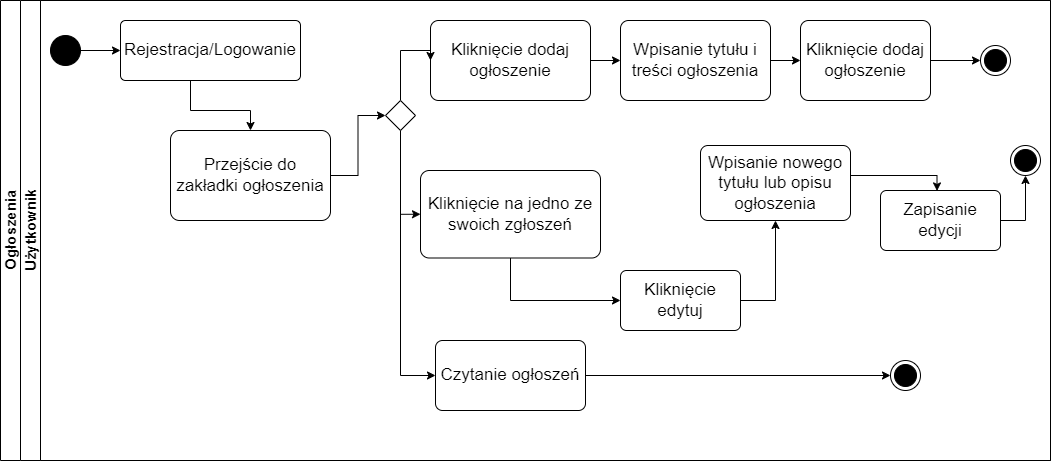
\includegraphics[width=1\linewidth]{img/ogloszenia_diag.png}
    \caption{Diagram procesu związanego z ogłoszeniami}
    \label{fig:posts-diag}
\end{figure}
\subsubsection{Dodanie pracownika}
Diagram prezentuje dodawanie nowego pracownika, z podziałem na 2 perspektywy: pracownika i administratora.
\begin{figure}[H]
    \centering
    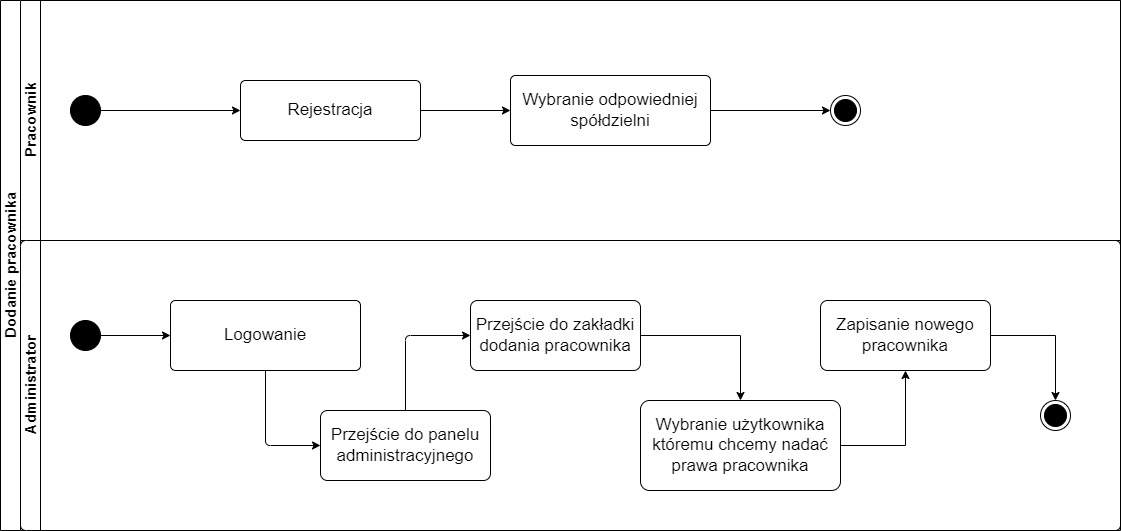
\includegraphics[width=1\linewidth]{img/prac_dod_diag.png}
    \caption{Diagram procesu dodania pracownika}
    \label{fig:add-worker-diag}
\end{figure}
\subsubsection{Zgłoszenia}
Diagram prezentuje operacje związane ze zgłoszeniami, w podziale na na 3 perspektywy: pracownika, mieszkańca oraz administratora. Dodana jest również perspektywa generycznego użytkownika z operacjami, które wykonać może każdy z typów użytkowników.
\begin{figure}
    \centering
    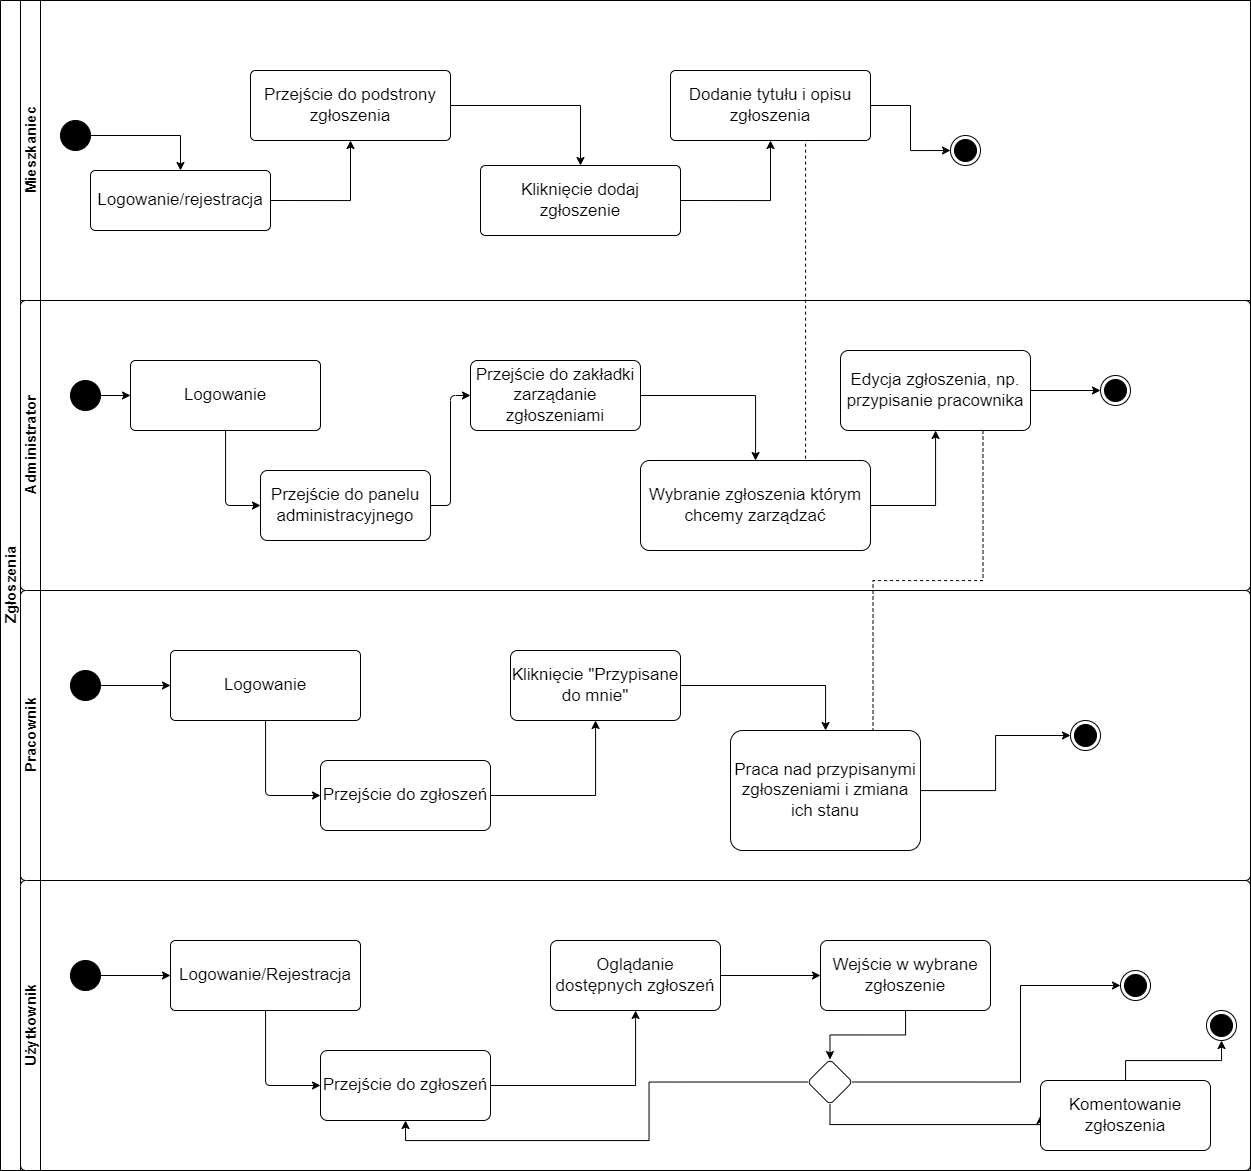
\includegraphics[width=1\linewidth]{img/use_case_requests.png}
    \caption{Diagram procesów związanych z zgłoszeniami}
    \label{fig:request-diag}
\end{figure}